% =============================================================================
% report.tex -- Data Analytics semestral project, topic: Specialty Cafes
% Every number in this file comes from the R scripts in analysis/: tables and
% figures are \input / \includegraphics, and numbers quoted in the text are
% macros defined in tables/results_macros.tex (written by 03_analysis.R).
% Compile from the report/ folder:  latexmk -pdf report.tex
% =============================================================================
\documentclass[11pt,a4paper]{article}

\usepackage[T1]{fontenc}
\usepackage[utf8]{inputenc}
\usepackage{newpxtext,newpxmath}
\usepackage[margin=2.5cm]{geometry}
\usepackage{amsmath}
\usepackage{booktabs}
\usepackage{graphicx}
\usepackage{adjustbox}
\usepackage{array}
\usepackage{float}
\usepackage[labelfont=bf,labelsep=period,font=small]{caption}
\usepackage{titlesec}
\usepackage[hidelinks]{hyperref}

\graphicspath{{figures/}}
\titleformat{\section}{\large\bfseries}{\thesection.}{0.6em}{}
\titleformat{\subsection}{\normalsize\bfseries}{\thesubsection}{0.6em}{}
\setlength{\parskip}{0.35em}

% ---- Reporting macros (same format everywhere) ------------------------------
\newcommand{\meanci}[4]{$M = #1$\,#4, 95\%~CI [#2, #3]}
\newcommand{\mdiffci}[4]{$M_\Delta = #1$\,#4, 95\%~CI [#2, #3]}
\newcommand{\diffci}[7]{$M_\Delta = #1$\,#4, 95\%~CI [#2, #3], $d = #5$, 95\%~CI [#6, #7]}
\newcommand{\dci}[3]{$d = #1$, 95\%~CI [#2, #3]}
\newcommand{\tstat}[2]{$t(#1) = #2$}
\newcommand{\pval}[1]{$p = #1$}
\newcommand{\plt}[1]{$p < #1$}
\newcommand{\Fstat}[3]{$F(#1, #2) = #3$}

% Written by analysis/03_analysis.R -- do not edit by hand.
\newcommand{\BenchCZK}{86.58}
\newcommand{\USDCZK}{21.646}
\newcommand{\Nall}{189}
\newcommand{\Nfilter}{54}
\newcommand{\Boot}{5,000}
\newcommand{\Seed}{2026}
\newcommand{\AoneN}{54}
\newcommand{\AoneEst}{\meanci{84.5}{80.3}{88.7}{CZK}}
\newcommand{\AoneDiff}{\mdiffci{\ensuremath{-}2.1}{\ensuremath{-}6.3}{2.1}{CZK}}
\newcommand{\AoneD}{\dci{\ensuremath{-}0.14}{\ensuremath{-}0.40}{0.13}}
\newcommand{\AoneT}{\tstat{53}{\ensuremath{-}1.00}, \pval{.321}}
\newcommand{\AoneMedian}{85.0}
\newcommand{\AoneWil}{$V = 590$, \pval{.190}}
\newcommand{\AoneBoot}{84.5 [80.6, 88.6]}
\newcommand{\AtwoNone}{54}
\newcommand{\AtwoNzero}{133}
\newcommand{\AtwoMone}{67.4}
\newcommand{\AtwoMzero}{63.5}
\newcommand{\AtwoEst}{\diffci{3.9}{0.1}{7.7}{CZK}{0.32}{0.00}{0.63}}
\newcommand{\AtwoT}{\tstat{105.5}{2.02}, \pval{.023} (one-tailed)}
\newcommand{\AtwoLower}{0.7}
\newcommand{\AtwoWil}{$W = 4370$, \pval{.010} (one-tailed)}
\newcommand{\AtwoHL}{5.0 [0.0, 7.0]}
\newcommand{\AtwoBoot}{3.9 [0.2, 7.6]}
\newcommand{\AtwoLevene}{\Fstat{1}{185}{0.17}, \pval{.682}}
\newcommand{\AthreeN}{54}
\newcommand{\AthreeEst}{\meanci{17.1}{13.9}{20.4}{CZK}}
\newcommand{\AthreeDz}{$d_z = 1.45$, 95\% CI [1.06, 1.83]}
\newcommand{\AthreeT}{\tstat{53}{10.65}, \plt{.001} (one-tailed)}
\newcommand{\AthreeMedian}{15.0}
\newcommand{\AthreeZero}{2}
\newcommand{\AthreeMax}{75}
\newcommand{\AthreeTrim}{16.0 [13.6, 18.5]}
\newcommand{\AthreeWil}{$V = 1378$, \plt{.001} (one-tailed)}
\newcommand{\AthreeBoot}{17.1 [14.3, 20.3]}
\newcommand{\AfourN}{187}
\newcommand{\AfourMNone}{\meanci{63.5}{61.2}{65.8}{CZK}}
\newcommand{\AfourNNone}{125}
\newcommand{\AfourMOne}{\meanci{66.2}{63.0}{69.5}{CZK}}
\newcommand{\AfourNOne}{49}
\newcommand{\AfourMBoth}{\meanci{69.3}{62.6}{76.0}{CZK}}
\newcommand{\AfourNBoth}{13}
\newcommand{\AfourF}{\Fstat{2}{33.1}{2.12}, \pval{.136}}
\newcommand{\AfourEta}{$\eta^2 = 0.020$, 95\% CI [0.000, 0.069]}
\newcommand{\AfourClassic}{\Fstat{2}{184}{1.89}, \pval{.153}}
\newcommand{\AfourLevene}{\Fstat{2}{184}{0.74}, \pval{.476}}
\newcommand{\AfourKW}{$H(2) = 6.42$, \pval{.040}}
\newcommand{\AfourGHOneNone}{$M_\Delta = 2.8$~CZK, 95\% CI [\ensuremath{-}1.9, 7.5], $p_{\text{adj}} = .339$}
\newcommand{\AfourGHBothNone}{$M_\Delta = 5.8$~CZK, 95\% CI [\ensuremath{-}2.6, 14.3], $p_{\text{adj}} = .206$}
\newcommand{\AfourGHBothOne}{$M_\Delta = 3.1$~CZK, 95\% CI [\ensuremath{-}5.7, 11.8], $p_{\text{adj}} = .654$}
\newcommand{\AfiveN}{187}
\newcommand{\AfiveRoast}{13 of 21 (61.9\%)}
\newcommand{\AfiveOther}{41 of 166 (24.7\%)}
\newcommand{\AfivePP}{37.2 percentage points, 95\% CI [15.4, 59.0]}
\newcommand{\AfiveChi}{$\chi^2(1, N = 187) = 12.56$, \plt{.001}}
\newcommand{\AfiveMinExp}{6.1}
\newcommand{\AfiveV}{$V = 0.26$, 95\% CI [0.09, 0.41]}
\newcommand{\AfiveRes}{3.54}
\newcommand{\AfiveFisher}{$\text{OR} = 4.90$, 95\% CI [1.74, 14.69], \pval{.001}}
\newcommand{\AsixN}{54}
\newcommand{\AsixR}{$r = 0.64$, 95\% CI [0.46, 0.78]}
\newcommand{\AsixT}{\tstat{52}{6.08}, \plt{.001}}
\newcommand{\AsixRho}{$\rho = 0.73$, 95\% CI [0.56, 0.85], \plt{.001}}
\newcommand{\AsixTau}{$\tau = 0.60$, 95\% CI [0.45, 0.74], \plt{.001}}
\newcommand{\AsixBoot}{[0.48, 0.83]}
\newcommand{\AsixRsq}{0.42}
\newcommand{\AsevenN}{54}
\newcommand{\AsevenB}{$b = 8.42$~CZK per 10~CZK, robust 95\% CI [6.20, 10.65]}
\newcommand{\AsevenT}{\tstat{52}{7.60}, \plt{.001}}
\newcommand{\AsevenRsq}{0.416}
\newcommand{\AsevenInt}{27.7}
\newcommand{\AsevenClassic}{[5.65, 11.20]}
\newcommand{\AsevenBoot}{[6.47, 10.97]}
\newcommand{\AsevenInfl}{3}
\newcommand{\AsevenNoInfl}{$b = 8.01$, 95\% CI [6.01, 10.02]}
\newcommand{\AeightN}{187}
\newcommand{\AeightBone}{$b = 3.90$~CZK, robust 95\% CI [0.06, 7.74], \pval{.047}}
\newcommand{\AeightBtwo}{$b = 4.40$~CZK, robust 95\% CI [0.58, 8.22], \tstat{184}{2.27}, \pval{.024}}
\newcommand{\AeightDist}{$b = \ensuremath{-}1.73$~CZK per km, robust 95\% CI [\ensuremath{-}3.02, \ensuremath{-}0.44], \pval{.009}}
\newcommand{\AeightChange}{0.50}
\newcommand{\AeightChangePct}{13}
\newcommand{\AeightF}{\Fstat{1}{184}{6.53}, \pval{.011}}
\newcommand{\AeightFrob}{\Fstat{1}{184}{6.99}, \pval{.009}}
\newcommand{\AeightVIF}{1.01}
\newcommand{\AeightRsqOne}{0.020}
\newcommand{\AeightRsqTwo}{0.054}
\newcommand{\AeightLog}{$b = 4.65$, 95\% CI [0.89, 8.41]}
\newcommand{\AeightInfl}{10}
\newcommand{\AeightNoInfl}{$b = 4.12$, 95\% CI [0.87, 7.36]}
\newcommand{\AnineN}{54}
\newcommand{\AnineNind}{35}
\newcommand{\AnineNchain}{19}
\newcommand{\AnineB}{$b = \ensuremath{-}6.02$~CZK per 10~CZK, robust 95\% CI [\ensuremath{-}12.00, \ensuremath{-}0.05], \tstat{50}{\ensuremath{-}2.02}, \pval{.048}}
\newcommand{\AnineF}{\Fstat{1}{50}{4.00}, \pval{.051}}
\newcommand{\AnineFrob}{\Fstat{1}{50}{4.10}, \pval{.048}}
\newcommand{\AnineSind}{$b = 11.44$~CZK, 95\% CI [6.22, 16.65]}
\newcommand{\AnineSchain}{$b = 5.41$~CZK, 95\% CI [2.48, 8.34]}
\newcommand{\AnineRsq}{0.459}
\newcommand{\AnineInfl}{3}
\newcommand{\AnineNoInfl}{$b = \ensuremath{-}7.18$, 95\% CI [\ensuremath{-}12.49, \ensuremath{-}1.86]}
\newcommand{\AnineVIF}{1.23}
\newcommand{\AtenN}{187}
\newcommand{\AtenEvents}{54}
\newcommand{\AtenAME}{4.5 percentage points per km, 95\% CI [0.9, 8.1], $z = 2.43$, \pval{.015}}
\newcommand{\AtenOR}{$\text{OR} = 1.25$ per km, 95\% CI [1.04, 1.52]}
\newcommand{\AtenBoot}{[0.9, 7.9]}
\newcommand{\AtenLPM}{4.6 percentage points, 95\% CI [0.9, 8.3]}
\newcommand{\AtenInfl}{8}
\newcommand{\AtenNoInfl}{6.3 percentage points, 95\% CI [2.4, 10.2]}
\newcommand{\AtenPwest}{17}
\newcommand{\AtenPzero}{24}
\newcommand{\AtenPeast}{44}
\newcommand{\HolmSig}{4}
\newcommand{\RawSig}{8}
\newcommand{\BPseven}{.933}
\newcommand{\BPeight}{.093}
\newcommand{\BPnine}{.538}
\newcommand{\Rversion}{4.6.1}
\newcommand{\Versandwich}{3.1.3}
\newcommand{\Verlmtest}{0.9.40}
\newcommand{\Vercar}{3.1.5}
\newcommand{\Vermarginaleffects}{1.0.0}


% Wide tables shrink to the text width; narrow ones keep their size.
\newcommand{\fittable}[1]{\begin{adjustbox}{max width=\textwidth}\input{tables/#1}\end{adjustbox}}

\title{\textbf{Filter coffee in Prague caf\'es: priced close to 4 USD, about 17 CZK above an espresso, and offered mostly by roasteries}}
\author{Aidan Osbaugh\\[0.2em]
  {\small Data Analytics, Batch \textit{Specialty Cafes}}\\
  {\small Partner: \textit{Luca Richardson}}}
\date{\today}

\begin{document}
\maketitle

\begin{abstract}
\noindent
We analyse \Nall{} Prague caf\'es whose menus were recorded by students in the class, \Nfilter{} of which sell filter coffee. A filter coffee cost $M = 84.5$\,CZK on average, not detectably different from the price of 4 USD (\BenchCZK\,CZK). In the same caf\'e it cost 17.1\,CZK more than an espresso (95\%~CI [13.9, 20.4]), and its price rose by 8.4\,CZK for every 10\,CZK of espresso price. Roasteries offered filter coffee far more often than other caf\'es (61.9\% vs 24.7\%, a difference of 37.2 percentage points). Caf\'es with filter coffee charged about 4\,CZK more for an espresso, and the chance that a caf\'e offers filter coffee grew by 4.5 percentage points per km east of the Old Town Square; these smaller effects do not survive a correction for ten tests.
\end{abstract}

% =============================================================================
\section{Introduction}

Filter coffee (pour-over or batch brew) is one of the visible markers of a ``specialty'' caf\'e: it needs better beans, more equipment and trained staff, and it is sold mostly to customers who care about origin and roast. If filter coffee signals a specialty caf\'e, caf\'es that offer it should look different from other caf\'es in what they charge, in whether they roast their own coffee, and perhaps in where they are located. We ask ten questions about Prague caf\'es (A1--A10 of the Specialty Caf\'es topic): what a filter coffee costs compared with the international benchmark of 4 US dollars and with an espresso in the same caf\'e; whether caf\'es that offer filter coffee, or that have more specialty features, charge more for an espresso; whether roasteries are more likely to offer filter coffee; how closely the filter and espresso prices of a caf\'e move together, and whether that link differs between independent caf\'es and chains; and whether filter coffee is more common east of the historic centre.

% =============================================================================
\section{Data and methods}

\subsection{Data}

The data were collected in person by the students of the class: for each caf\'e, the price of an espresso, cappuccino, flat white and filter coffee (from the menu, with a photo as evidence), the type of caf\'e, whether it roasts its own coffee, and its coordinates. The raw sheet has 299 rows; \texttt{01\_cleaning.R} turns it into an analysis dataset of \Nall{} caf\'es (Table~\ref{tab:cleaning}). It drops 99 empty rows at the bottom of the sheet and 11 caf\'es that two students entered twice (found as pairs less than 50\,m apart and confirmed by name and address; the more complete entry is kept). It harmonises 17 district labels, sets one blank caf\'e type to missing, removes the thousands separator from 4 rating counts, and, where a cell holds several prices (sizes, dine-in/take-away), keeps the first price, which is the smallest size or the dine-in price (espresso 11 caf\'es, filter coffee 8).

The filter price has three meanings that the analysis depends on: a price means the caf\'e offers filter coffee, ``NA'' means it does not (133 caf\'es), and a blank means we do not know (2 caf\'es, set to missing). Hence the filter price is available for \Nfilter{} caf\'es, the indicator ``offers filter coffee'' for 187, and the espresso price, the roastery indicator and the distance from the Orloj (the astronomical clock on the Old Town Square) for all \Nall. Caf\'e type is missing for one caf\'e, which does not sell filter coffee, so A9 is unaffected. No variable was log-transformed for the main analyses: the prices are moderately right-skewed but the samples are large enough for the central limit theorem (Appendix~\ref{app:distributions}); a log of the distance is used as a robustness check in A8. The full descriptive statistics are in Appendix~\ref{app:descriptives}.

\begin{table}[H]
\centering\small
\caption{Cleaning steps applied by \texttt{01\_cleaning.R} and the number of caf\'es affected.}
\label{tab:cleaning}
\begin{tabular}{lr}
\toprule
Cleaning step & Caf\'es \\
\midrule
Rows in the raw file & 299 \\
Leading or trailing spaces removed (rows) & 62 \\
Empty rows dropped & 99 \\
Exactly duplicated rows dropped & 0 \\
Same cafe entered twice: second entry dropped & 11 \\
Cafes after removing empty and duplicate rows & 189 \\
District labels harmonised & 17 \\
Blank cafe type set to missing & 1 \\
Several prices, first kept: espresso & 11 \\
Several prices, first kept: cappuccino & 11 \\
Several prices, first kept: flatwhite & 3 \\
Several prices, first kept: filter & 8 \\
Filter price blank: offers filter set to missing & 2 \\
Flat white marked NA (not served) & 2 \\
Thousands separator removed (number of ratings) & 4 \\
Cafes in the analysis dataset & 189 \\
\bottomrule
\end{tabular}

\end{table}

\subsection{Statistical methods}

All tests use $\alpha = .05$. Hypotheses and their direction were fixed before the data were analysed (they are written at the top of \texttt{03\_analysis.R}); A2 and A3 are one-tailed because the questions name a direction, all others two-tailed. The method for each question was chosen in \texttt{02\_descriptive.R} from the histograms, Q--Q plots, the skewness and the group sizes (Appendix~\ref{app:distributions}): every compared variable is either close to normal or large enough ($n \ge 49$) for its mean to be approximately normal, so the parametric method is used for every question and only its result is reported in the main text. We use a one-sample $t$-test (A1), Welch's $t$-test (A2), a paired $t$-test (A3), Welch's one-way ANOVA with Games--Howell post hoc comparisons, chosen because the groups are very unequal in size (A4), Pearson's $\chi^2$ test without continuity correction (A5), Pearson's correlation (A6), ordinary least squares with HC3 heteroskedasticity-robust standard errors (A7--A9), and logistic regression with the average marginal effect and its delta-method interval (A10). Confidence intervals of means are $t$-based; those of Cohen's $d$ and $\eta^2$ use the noncentral $t$ and $F$ distributions; bootstrap intervals are percentile intervals from \Boot{} resamples with seed \Seed. Other assumptions were checked for each method: the equality of variances with Levene's test before comparing groups (A2, A4), the expected counts of the contingency table (A5), and the residuals and influential observations of every regression (A7--A10, Appendix~\ref{app:diagnostics}). Multiple comparisons within A4 are adjusted by the Games--Howell procedure. Every test assumes that caf\'es are independent, but caf\'es in the same district share rents and customers; their prices are therefore positively correlated, which makes the standard errors too small and the $p$-values too low, so results near $p = .05$ deserve particular caution. The rank-based, bootstrap and other checks in Appendix~\ref{app:robustness} were not planned in advance and are exploratory. The analysis was run in R~\Rversion{} with the packages \texttt{sandwich}~\Versandwich, \texttt{lmtest}~\Verlmtest, \texttt{car}~\Vercar{} and \texttt{marginaleffects}~\Vermarginaleffects.

% =============================================================================
\section{Results}

Table~\ref{tab:summary} summarises the main result of every analysis; the subsections below give the details.

\begin{table}[H]
\centering\small
\caption{Main results of the ten analyses. Estimates in the original units with 95\% confidence intervals; pp = percentage points; $p$ is one-tailed for A2 and A3 and two-tailed otherwise. A4 shows the largest pairwise difference. Lost = caf\'es of the \Nall{} excluded because of missing values (no filter price, or unknown filter status).}
\label{tab:summary}
\fittable{summary.tex}
\end{table}

% -----------------------------------------------------------------------------
\subsection{A1: Filter coffee price against 4 US dollars}

\emph{Is the average price of a filter coffee different from 4 USD?} The benchmark was fixed before looking at the data: 4 USD at the Czech National Bank rate of 5 November 2026 (\USDCZK\,CZK per USD) is \BenchCZK\,CZK. $H_0$: $\mu = \BenchCZK$\,CZK; $H_1$: $\mu \neq \BenchCZK$\,CZK.

Figure~\ref{fig:A1} shows the \AoneN{} filter prices; most lie between 75 and 90\,CZK with a few expensive cups up to 145\,CZK. The mean price was \AoneEst, so the difference from the benchmark was \AoneDiff, with \AoneD. A one-sample $t$-test gave \AoneT. The median price was \AoneMedian\,CZK (Table~\ref{tab:A1}). The 135 caf\'es without a filter price (133 not offering filter coffee, 2 unknown) are not part of this analysis. In this sample, a filter coffee in Prague costs about what 4 USD buys: the data are compatible with a price between 6\,CZK below and 2\,CZK above the benchmark.

\begin{figure}[H]
\centering
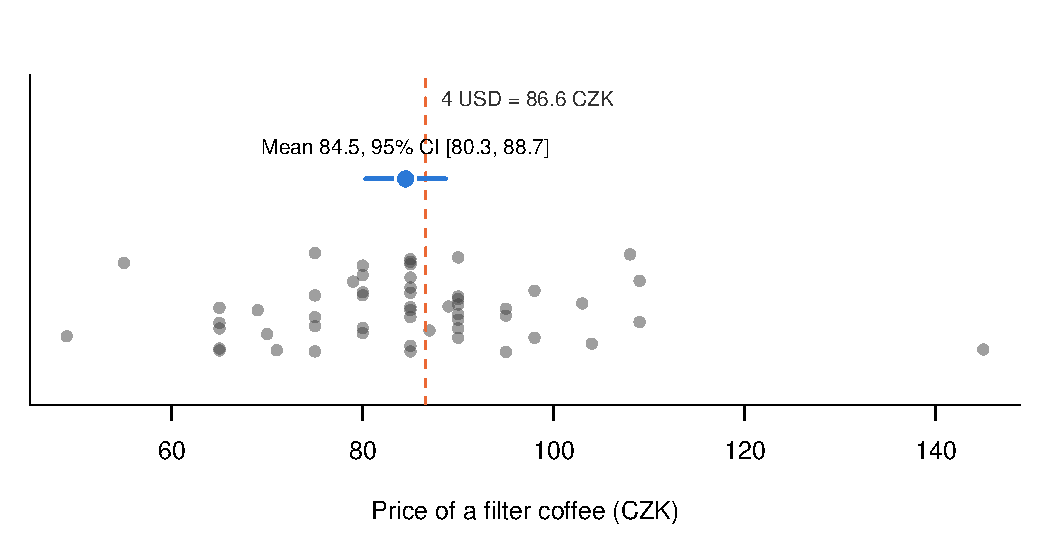
\includegraphics[width=0.85\textwidth]{A1_figure.pdf}
\caption{Price of a filter coffee in the \AoneN{} caf\'es that offer it (CZK; grey points, vertically jittered). The blue point and bar show the mean with its 95\% confidence interval; the dashed line is the benchmark of 4 USD = \BenchCZK\,CZK.}
\label{fig:A1}
\end{figure}

\begin{table}[H]
\centering\small
\caption{A1: mean filter coffee price (CZK) with its 95\% confidence interval, the difference from the benchmark of \BenchCZK\,CZK, Cohen's $d$, and the one-sample $t$-test (two-tailed).}
\label{tab:A1}
\fittable{A1_table.tex}
\end{table}

% -----------------------------------------------------------------------------
\subsection{A2: Espresso price in caf\'es with and without filter coffee}

\emph{Do caf\'es that offer filter coffee charge more for an espresso than caf\'es that do not?} The difference is the mean espresso price of caf\'es that offer filter coffee \emph{minus} that of caf\'es that do not. $H_0$: $\mu_1 - \mu_0 = 0$; $H_1$: $\mu_1 - \mu_0 > 0$ (one-tailed).

Figure~\ref{fig:A2} shows the two groups. The \AtwoNone{} caf\'es with filter coffee charged on average \AtwoMone\,CZK for an espresso, the \AtwoNzero{} caf\'es without it \AtwoMzero\,CZK: \AtwoEst. Welch's test gave \AtwoT; the one-sided 95\% lower bound of the difference is \AtwoLower\,CZK. Levene's test gave no evidence of unequal variances (\AtwoLevene); Welch's test does not need equal variances in any case. Two caf\'es with unknown filter status were lost (Table~\ref{tab:A2}). (The interval of $d$ uses the pooled standard deviation and therefore just touches zero, while the Welch interval of the raw difference does not.) In this sample, caf\'es that offer filter coffee charge about 4\,CZK more for an espresso, a small effect.

\begin{figure}[H]
\centering
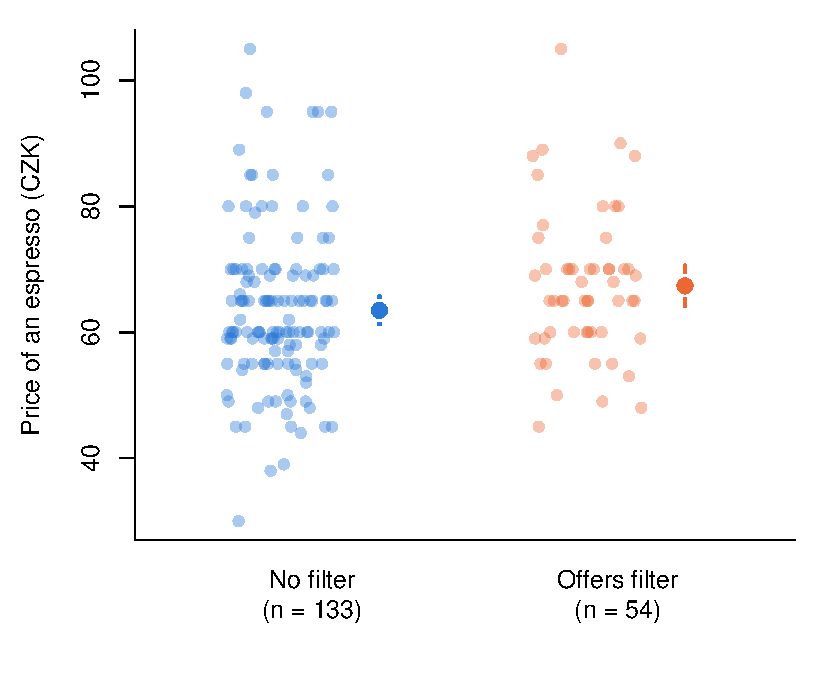
\includegraphics[width=0.6\textwidth]{A2_figure.pdf}
\caption{Price of an espresso (CZK) in caf\'es that do not and that do offer filter coffee. Faint points are individual caf\'es (jittered); the solid point and bar show the group mean and its 95\% confidence interval. Two caf\'es with unknown filter status are excluded.}
\label{fig:A2}
\end{figure}

\begin{table}[H]
\centering\small
\caption{A2: difference in mean espresso price (CZK), caf\'es offering filter coffee minus caf\'es that do not, with its two-sided 95\% confidence interval, Cohen's $d$, and Welch's $t$-test. The $p$-value is one-tailed, as fixed in advance.}
\label{tab:A2}
\fittable{A2_table.tex}
\end{table}

% -----------------------------------------------------------------------------
\subsection{A3: Filter coffee against espresso in the same caf\'e}

\emph{How much more does a filter coffee cost than an espresso in the same caf\'e?} The within-caf\'e difference is the filter price \emph{minus} the espresso price. $H_0$: $\mu_d = 0$; $H_1$: $\mu_d > 0$ (one-tailed).

Figure~\ref{fig:A3} shows the \AthreeN{} differences. Only \AthreeZero{} caf\'es charge the same for both, and none charges less for filter coffee; one caf\'e charges \AthreeMax\,CZK more. The mean difference was \AthreeEst{} (median \AthreeMedian\,CZK), \AthreeDz, \AthreeT. The 135 caf\'es without a filter price were lost (Table~\ref{tab:A3}). In this sample, a filter coffee costs about 17\,CZK more than an espresso in the same caf\'e, a large and consistent difference.

\begin{figure}[H]
\centering
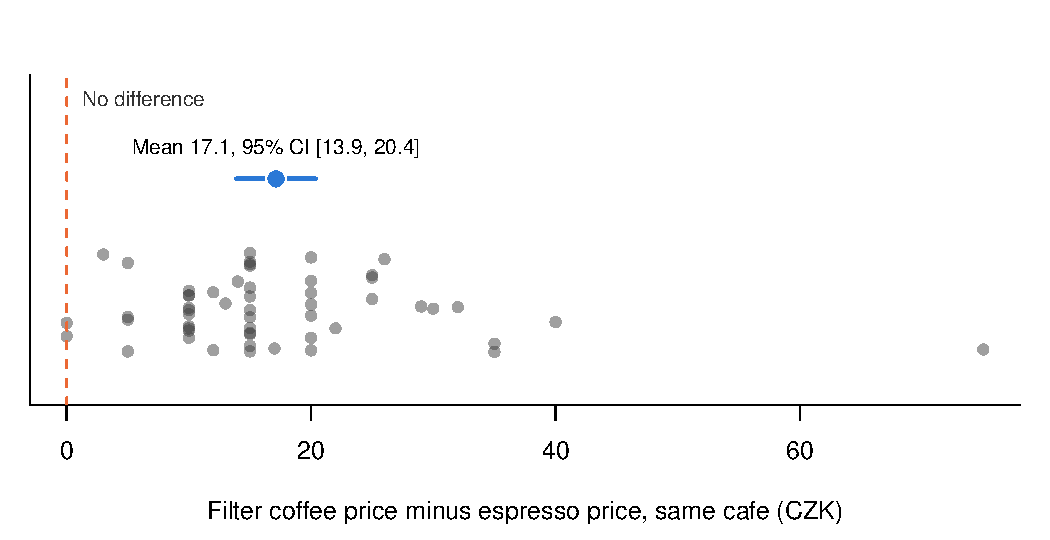
\includegraphics[width=0.85\textwidth]{A3_figure.pdf}
\caption{Filter coffee price minus espresso price in the same caf\'e (CZK) for the \AthreeN{} caf\'es that sell both (grey points, vertically jittered). The blue point and bar show the mean difference with its 95\% confidence interval; the dashed line marks no difference. The two prices of each caf\'e are shown in Figure~\ref{fig:paired} in Appendix~\ref{app:distributions}.}
\label{fig:A3}
\end{figure}

\begin{table}[H]
\centering\small
\caption{A3: mean within-caf\'e difference, filter coffee minus espresso (CZK), with its two-sided 95\% confidence interval, median and IQR, $d_z$, and the paired $t$-test. The $p$-value is one-tailed, as fixed in advance.}
\label{tab:A3}
\fittable{A3_table.tex}
\end{table}

% -----------------------------------------------------------------------------
\subsection{A4: Espresso price by number of specialty features}

\emph{Does the espresso price differ between caf\'es with none, one or both specialty features (being a roastery, offering filter coffee)?} $H_0$: $\mu_\text{none} = \mu_\text{one} = \mu_\text{both}$; $H_1$: at least one mean differs.

The mean espresso price rose with the number of features (Figure~\ref{fig:A4}): none \AfourMNone{} ($n = \AfourNNone$), one \AfourMOne{} ($n = \AfourNOne$), both \AfourMBoth{} ($n = \AfourNBoth$). Levene's test gave no evidence of unequal variances (\AfourLevene), but the groups are very unequal in size, so Welch's ANOVA was used: \AfourF, with \AfourEta. Two caf\'es with unknown filter status were lost. None of the Games--Howell comparisons was significant (Table~\ref{tab:A4}); the largest, both minus none, was \AfourGHBothNone. In this sample the espresso price tends to rise with the number of specialty features, by about 6\,CZK from none to both, but there is no evidence of a difference: the groups are small and variable, especially the 13 caf\'es with both features; at most about 7\% of the variation in espresso prices is linked to the features.

\begin{figure}[H]
\centering
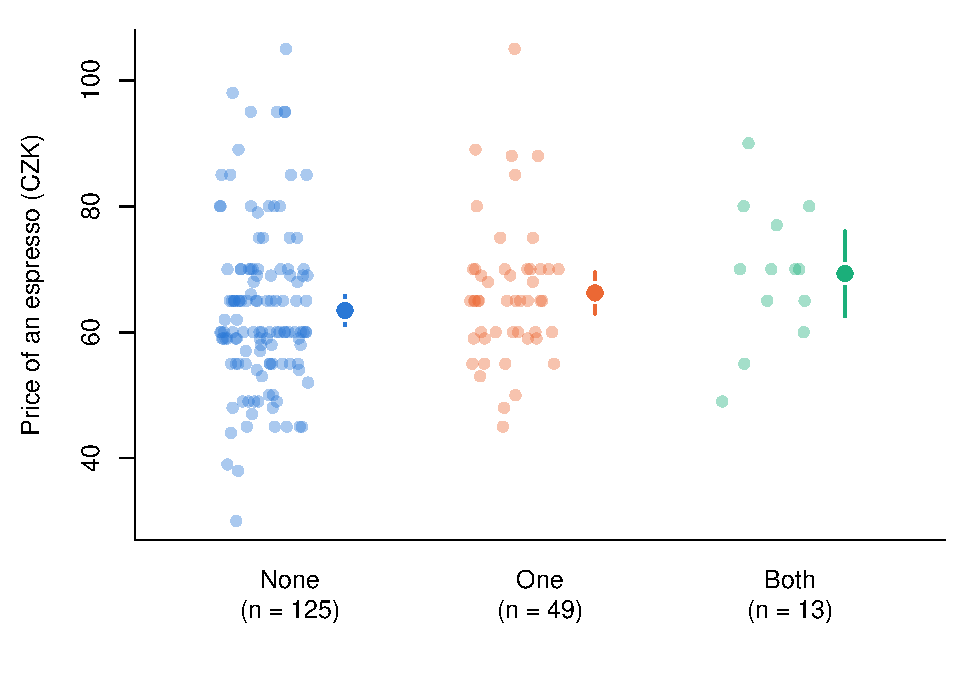
\includegraphics[width=0.7\textwidth]{A4_figure.pdf}
\caption{Price of an espresso (CZK) by the number of specialty features of the caf\'e (roastery, filter coffee). Faint points are individual caf\'es (jittered); solid points and bars are group means with 95\% confidence intervals. Two caf\'es with unknown filter status are excluded ($N = \AfourN$).}
\label{fig:A4}
\end{figure}

\begin{table}[H]
\centering\small
\caption{A4: Games--Howell pairwise comparisons of the mean espresso price (CZK). Differences with simultaneous 95\% confidence intervals and adjusted $p$-values; the omnibus test is in the last row.}
\label{tab:A4}
\fittable{A4_table.tex}
\end{table}

% -----------------------------------------------------------------------------
\subsection{A5: Roasteries and filter coffee}

\emph{Is a roastery more likely to offer filter coffee than other caf\'es, and by how many percentage points?} $H_0$: offering filter coffee is independent of being a roastery; $H_1$: the two are associated (two-sided test). The difference is roasteries \emph{minus} other caf\'es.

Table~\ref{tab:A5} and Figure~\ref{fig:A5} show the counts. \AfiveRoast{} roasteries offered filter coffee, against \AfiveOther{} other caf\'es: a difference of \AfivePP. The $\chi^2$ test gave \AfiveChi; the smallest expected count was \AfiveMinExp, so no expected count is below 5 and the $\chi^2$ test is appropriate. Two caf\'es with unknown filter status were lost. The association was moderate, \AfiveV. The cell that departs most from independence is roasteries offering filter coffee (standardised residual \AfiveRes). In this sample, a roastery is about two and a half times as likely as another caf\'e to offer filter coffee.

\begin{table}[H]
\centering\small
\caption{A5: caf\'es by roastery status and whether they offer filter coffee: counts with row percentages, and the standardised residuals of the ``offers filter'' column ($N = \AfiveN$).}
\label{tab:A5}
\fittable{A5_table.tex}
\end{table}

\begin{figure}[H]
\centering
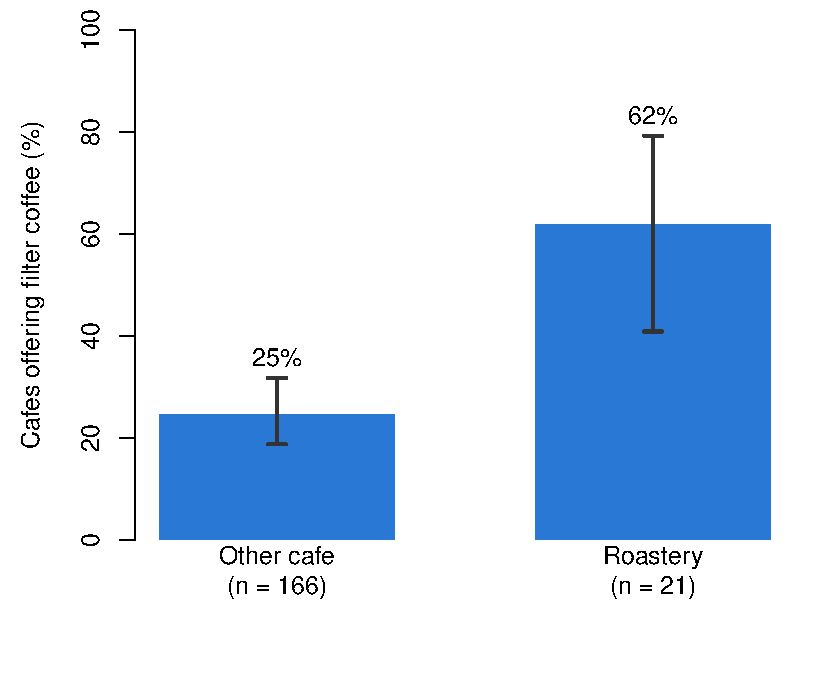
\includegraphics[width=0.55\textwidth]{A5_figure.pdf}
\caption{Share of caf\'es offering filter coffee (\%) among other caf\'es and roasteries, with 95\% Wilson confidence intervals. Two caf\'es with unknown filter status are excluded.}
\label{fig:A5}
\end{figure}

% -----------------------------------------------------------------------------
\subsection{A6: Correlation of filter coffee and espresso prices}

\emph{Is the filter coffee price correlated with the espresso price, and in which direction and how strongly?} $H_0$: $\rho = 0$; $H_1$: $\rho \neq 0$.

Figure~\ref{fig:A6} shows a clear positive, roughly linear relation among the \AsixN{} caf\'es with both prices. Pearson's correlation was \AsixR, \AsixT{} (Table~\ref{tab:A6}): the two prices share $r^2 = \AsixRsq$ of their variance. In this sample, caf\'es with a more expensive espresso also have a more expensive filter coffee, and the association is strong; it says nothing about why.

\begin{figure}[H]
\centering
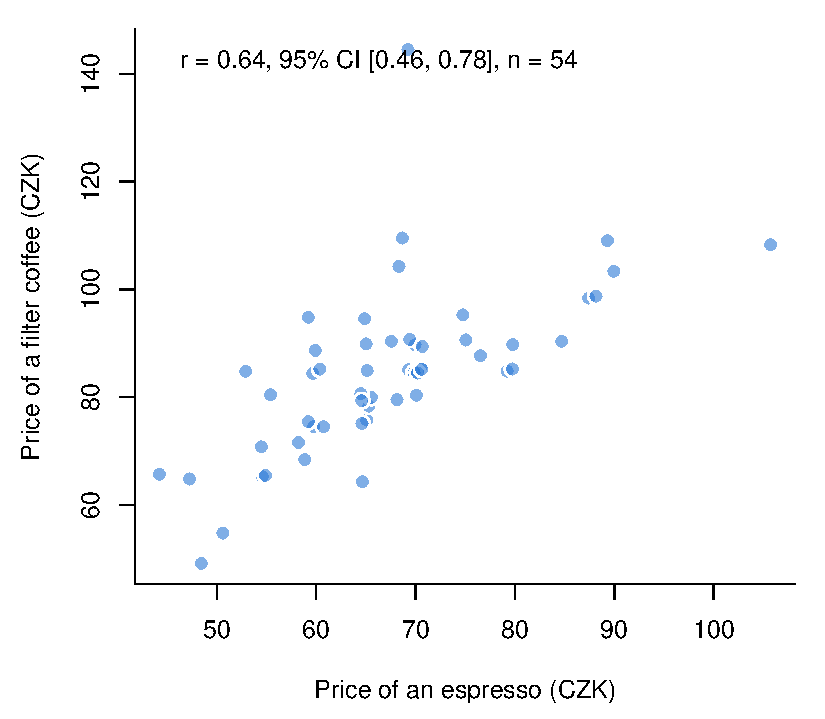
\includegraphics[width=0.55\textwidth]{A6_figure.pdf}
\caption{Price of a filter coffee against the price of an espresso in the same caf\'e (CZK), $n = \AsixN$. The legend gives Pearson's $r$ with its 95\% confidence interval. Points are slightly jittered because many prices are round numbers.}
\label{fig:A6}
\end{figure}

\begin{table}[H]
\centering\small
\caption{A6: Pearson correlation of the filter coffee and espresso price with its 95\% confidence interval (Fisher $z$), the shared variance $r^2$, and the two-tailed test.}
\label{tab:A6}
\fittable{A6_table.tex}
\end{table}

% -----------------------------------------------------------------------------
\subsection{A7: Filter coffee price per 10 CZK of espresso price}

\emph{By how many CZK does the filter coffee price change per 10\,CZK increase in the espresso price?} Model: filter price $= b_0 + b_1 \cdot$ (espresso price / 10) $+ e$. $H_0$: $b_1 = 0$; $H_1$: $b_1 \neq 0$.

The fitted line (Figure~\ref{fig:A7}, Table~\ref{tab:A7}) has slope \AsevenB, \AsevenT, with $R^2 = \AsevenRsq$. The residual plots (Figure~\ref{fig:diag}) show no curvature and no funnel (Breusch--Pagan $p = \BPseven$), the residuals have a slightly long right tail from a few expensive filter coffees, and \AsevenInfl{} caf\'es have a large Cook's distance; without them the slope is \AsevenNoInfl, so they do not change the conclusion. The residual spread is constant, so the robust standard errors barely differ from the classical ones. In this sample, a caf\'e whose espresso costs 10\,CZK more charges on average about 8\,CZK more for a filter coffee, and the espresso price accounts for about 42\% of the variation in filter prices.

\begin{figure}[H]
\centering
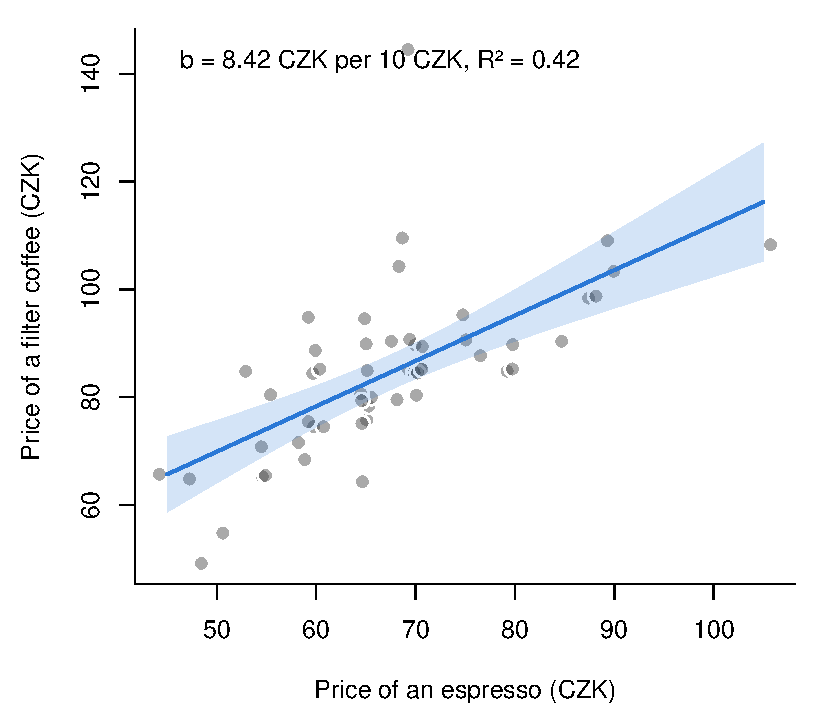
\includegraphics[width=0.55\textwidth]{A7_figure.pdf}
\caption{Price of a filter coffee against the price of an espresso (CZK), $n = \AsevenN$, with the least-squares line and its 95\% confidence band. Points are slightly jittered.}
\label{fig:A7}
\end{figure}

\begin{table}[H]
\centering\small
\caption{A7: regression of the filter coffee price (CZK) on the espresso price in units of 10\,CZK, with HC3 robust standard errors and confidence intervals ($n = \AsevenN$).}
\label{tab:A7}
\fittable{A7_table.tex}
\end{table}

% -----------------------------------------------------------------------------
\subsection{A8: The filter coffee gap after accounting for distance}

\emph{Does the espresso price differ between caf\'es that offer filter coffee and those that do not once we account for the distance from the Orloj?} Model~1: espresso price $= b_0 + b_1\cdot$filter $+ e$; Model~2 adds the distance in km. $H_0$: $b_1 = 0$ in Model~2; $H_1$: $b_1 \neq 0$.

Table~\ref{tab:A8} shows both models. Without distance the gap was \AeightBone{} (the same 3.9\,CZK as in A2). With distance, the gap was \AeightBtwo, and the espresso price fell with distance from the centre, \AeightDist{} (Figure~\ref{fig:A8}). The nested $F$-test favours Model~2, \AeightF{} (robust Wald test \AeightFrob), although $R^2$ rises only from \AeightRsqOne{} to \AeightRsqTwo. Accounting for distance \emph{increased} the gap by \AeightChange\,CZK (\AeightChangePct\%), because caf\'es with filter coffee lie on average a little further from the centre, where espressos are cheaper. The variance inflation factors are \AeightVIF, so the two predictors are practically unrelated. Without the \AeightInfl{} influential caf\'es the gap is \AeightNoInfl, so they do not drive the result (Appendix~\ref{app:diagnostics}). In this sample, among caf\'es at the same distance from the Orloj, those that offer filter coffee charge about 4.4\,CZK more for an espresso.

\begin{table}[H]
\centering\small
\caption{A8: regression of the espresso price (CZK) on offering filter coffee, without (Model~1) and with (Model~2) the distance from the Orloj. Estimates with HC3 robust standard errors in parentheses and robust 95\% confidence intervals below.}
\label{tab:A8}
\fittable{A8_table.tex}
\end{table}

\begin{figure}[H]
\centering
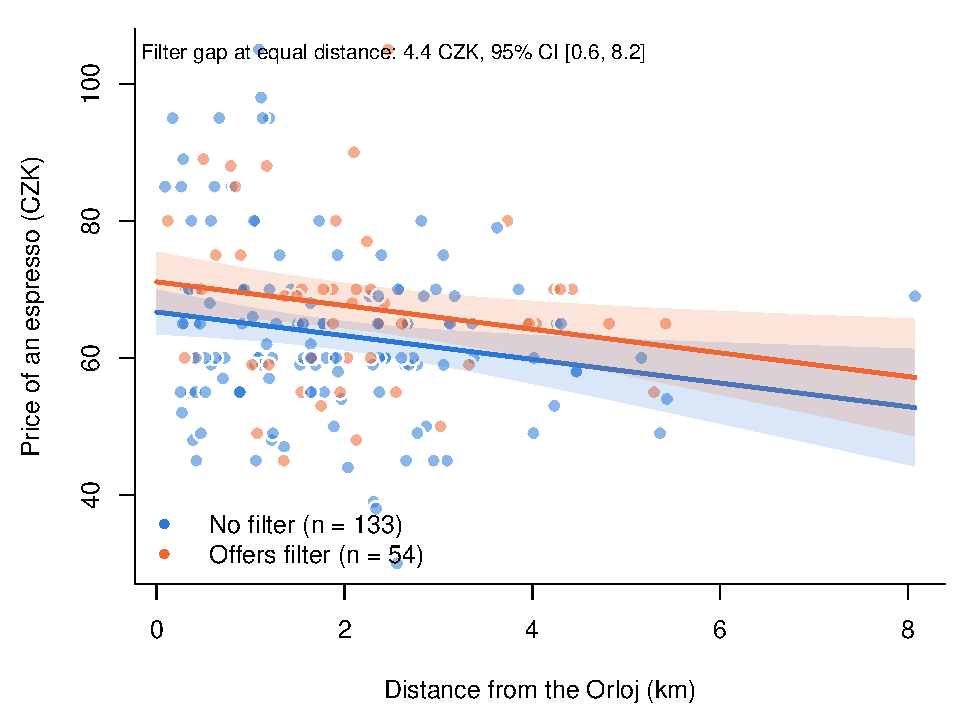
\includegraphics[width=0.68\textwidth]{A8_figure.pdf}
\caption{Price of an espresso (CZK) against the distance from the Orloj (km) for caf\'es without (blue) and with (orange) filter coffee, with the parallel lines of Model~2 and their 95\% confidence bands; the label gives the filter gap at equal distance ($N = \AeightN$).}
\label{fig:A8}
\end{figure}

% -----------------------------------------------------------------------------
\subsection{A9: Does the price link differ between independents and chains?}

\emph{Does the relationship between the espresso price and the filter coffee price differ between independent caf\'es and chains?} Model: filter price $= b_0 + b_1\cdot$espresso$/10 + b_2\cdot$chain $+ b_3\cdot$(espresso$/10 \times$ chain) $+ e$, where chain combines local and international chains. $H_0$: $b_3 = 0$; $H_1$: $b_3 \neq 0$.

Among the \AnineN{} caf\'es with filter coffee (\AnineNind{} independent, \AnineNchain{} chains), the interaction was \AnineB{} (Table~\ref{tab:A9}); the robust nested test gave \AnineFrob, the classic nested $F$-test \AnineF. Per 10\,CZK of espresso price, the filter price rose by \AnineSind{} in independent caf\'es and by \AnineSchain{} in chains (Figure~\ref{fig:A9}). Without the \AnineInfl{} influential caf\'es the interaction is \AnineNoInfl. In this sample, filter prices follow espresso prices about twice as steeply in independent caf\'es as in chains, but the evidence is borderline: the result sits on the threshold of $p = .05$ and depends on 19 chain caf\'es. (The chain coefficient $b_2$ describes an espresso price of 0\,CZK and has no meaning by itself.)

\begin{table}[H]
\centering\small
\caption{A9: regression of the filter coffee price (CZK) on the espresso price (per 10\,CZK), chain status and their interaction, with HC3 robust 95\% confidence intervals ($n = \AnineN$). The lower rows give the slope within each group.}
\label{tab:A9}
\fittable{A9_table.tex}
\end{table}

\begin{figure}[H]
\centering
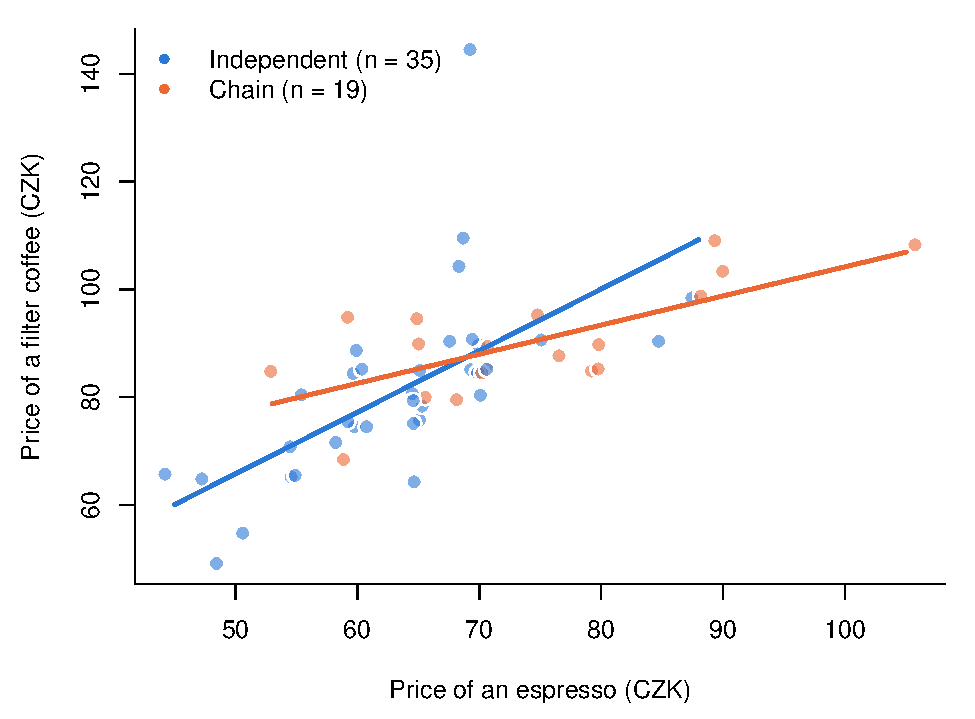
\includegraphics[width=0.68\textwidth]{A9_figure.pdf}
\caption{Price of a filter coffee against the price of an espresso (CZK) in independent caf\'es (blue, $n = \AnineNind$) and chains (orange, $n = \AnineNchain$), with the fitted line of the interaction model and its 95\% confidence band in each group over its observed range. Points are slightly jittered.}
\label{fig:A9}
\end{figure}

% -----------------------------------------------------------------------------
\subsection{A10: Filter coffee east of the Orloj}

\emph{Does the probability that a caf\'e offers filter coffee change with each additional km east of the Orloj, and by how many percentage points?} The binary outcome is the indicator created in cleaning: 1 if a filter price was recorded, 0 if the collector wrote ``NA''; the 2 caf\'es with a blank are excluded. The predictor is the east--west distance from the Orloj in km (positive = east, $(\text{longitude} - 14.4207) \times 71$). Model: $\operatorname{logit} P(\text{filter}) = b_0 + b_1\cdot$km east. $H_0$: the average marginal effect is 0; $H_1$: it is not 0.

Of the \AtenN{} caf\'es, \AtenEvents{} offer filter coffee. The average marginal effect of one km further east was \AtenAME. As a check, the odds ratio was \AtenOR{} (Table~\ref{tab:A10}). The predicted probability (Figure~\ref{fig:A10}) rises from \AtenPwest\% at 2\,km west of the Orloj to \AtenPzero\% at the Orloj and \AtenPeast\% at 4\,km east. Without the \AtenInfl{} influential caf\'es the effect is \AtenNoInfl, so the conclusion does not depend on them. In this sample, each km further east goes with a chance of offering filter coffee about 4.5 percentage points higher.

\begin{table}[H]
\centering\small
\caption{A10: logistic regression of offering filter coffee on the distance east of the Orloj (km), $n = \AtenN$, \AtenEvents{} events. The average marginal effect (delta-method interval) is the headline; the odds ratio (profile-likelihood interval) is a check; the linear probability model (HC3) is an exploratory check. pp = percentage points.}
\label{tab:A10}
\fittable{A10_table.tex}
\end{table}

\begin{figure}[H]
\centering
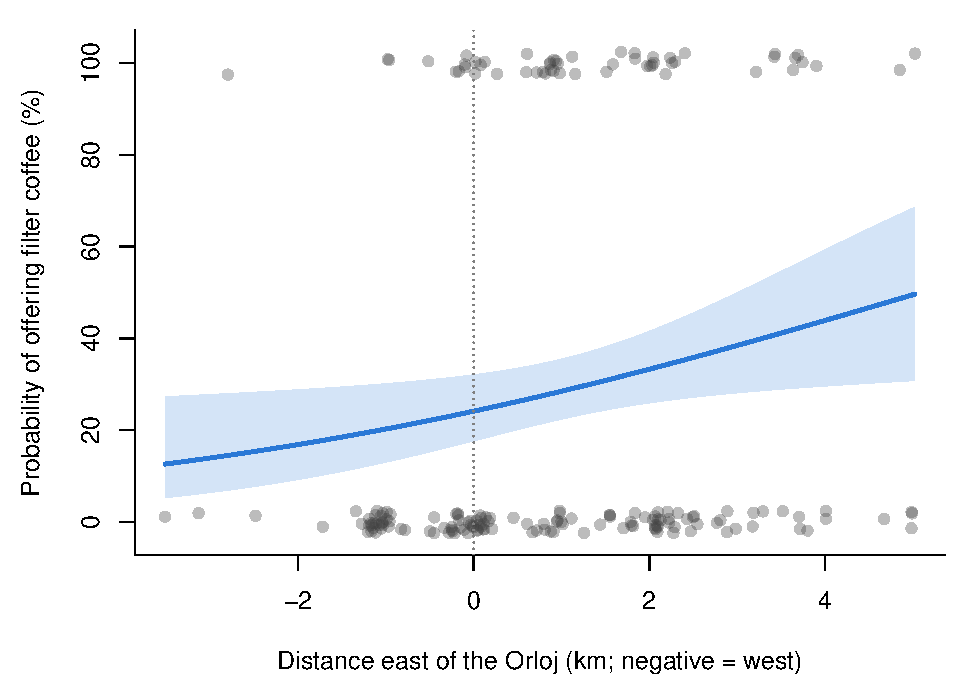
\includegraphics[width=0.68\textwidth]{A10_figure.pdf}
\caption{Predicted probability (\%) that a caf\'e offers filter coffee against the distance east of the Orloj (km; negative = west), from the logistic model, with its 95\% confidence band. Grey points are the \AtenN{} caf\'es at 0\% (no filter) or 100\% (filter), vertically jittered; the dotted line marks the Orloj.}
\label{fig:A10}
\end{figure}

% =============================================================================
\section{Discussion}

Taken together, the results draw a consistent picture of filter coffee in this sample of Prague caf\'es. Its price sits close to the international benchmark of 4 USD (A1) and about 17\,CZK above the espresso of the same caf\'e (A3); it tracks the caf\'e's espresso price closely (A6, A7), with about 8\,CZK more for filter per 10\,CZK more for espresso. Filter coffee is strongly concentrated in roasteries (A5). These four results are large, precise, and robust to every alternative method and to Holm's adjustment across the ten questions (Table~\ref{tab:holm}).

The remaining results are smaller and should be read as exploratory. Caf\'es that offer filter coffee charge about 4\,CZK more for an espresso (A2), a gap that holds after accounting for distance (A8); the espresso price tends to rise with the number of specialty features but not significantly (A4); filter prices may follow espresso prices less steeply in chains (A9); and filter coffee becomes more common further east (A10). A2, A8, A9 and A10 are significant only by a narrow margin, A4 and A9 change their verdict depending on the method, and none survives Holm's adjustment. They are plausible effects of modest size, not established findings.

A reader should not conclude more than the design allows. The caf\'es form a convenience sample chosen by students, with a strong concentration in central districts; it is not a random sample of Prague caf\'es, so averages may not hold for the city as a whole. The data are observational: offering filter coffee does not \emph{cause} higher espresso prices, and both are likely to reflect a caf\'e's positioning, rent and clientele. Caf\'es in the same district share rents and customers, so their prices are not independent of one another and our standard errors are probably too small. Prices were recorded from menus by different students, multi-price cells were reduced to the first price, and the filter price exists only for the 54 caf\'es that sell it, which limits A1, A3, A6, A7 and A9 to that group and leaves only 19 chains in A9. All conclusions are therefore stated for this sample.

\section{Conclusion}

What do specialty caf\'es in Prague offer? In this sample, filter coffee, the clearest specialty marker we recorded, is sold by fewer than a third of caf\'es, but by most roasteries. It costs about what 4 US dollars buy, about 17\,CZK more than an espresso in the same caf\'e, and caf\'es set its price in line with their espresso. Caf\'es that offer it charge slightly more for an espresso and are somewhat more common east of the centre, but these smaller differences are uncertain. Specialty caf\'es therefore stand out more in \emph{what} they offer than in what they charge for the basics.

% =============================================================================
\appendix
\renewcommand{\thesection}{\Alph{section}}
\titleformat{\section}{\large\bfseries}{\thesection.}{0.6em}{}

\section{Descriptive statistics}\label{app:descriptives}

Table~\ref{tab:descriptives} describes the numeric variables and Table~\ref{tab:categorical} the categorical ones, as produced by \texttt{02\_descriptive.R}. The filter price and the within-caf\'e difference are missing for the 135 caf\'es that do not offer filter coffee or whose status is unknown.

\begin{table}[H]
\centering\small
\caption{Descriptive statistics of the numeric variables used. Means are shown with 95\% confidence intervals; IQR is the first to the third quartile.}
\label{tab:descriptives}
\fittable{descriptives.tex}
\end{table}

\begin{table}[H]
\centering\small
\caption{Counts and percentages of the categorical variables used ($N = \Nall$).}
\label{tab:categorical}
\begin{tabular}{llrr}
\toprule
Variable & Category & n & Percent \\
\midrule
Offers filter coffee & No filter & 133 & 70.4 \\
 & Offers filter &  54 & 28.6 \\
 & Missing &   2 & 1.1 \\
Roastery & Other cafe & 167 & 88.4 \\
 & Roastery &  22 & 11.6 \\
 & Missing &   0 & 0.0 \\
Specialty features & None & 125 & 66.1 \\
 & One &  49 & 25.9 \\
 & Both &  13 & 6.9 \\
 & Missing &   2 & 1.1 \\
Cafe type & Independent & 131 & 69.3 \\
 & Local Chain &  48 & 25.4 \\
 & International Chain &   9 & 4.8 \\
 & Missing &   1 & 0.5 \\
Independent or chain & Independent & 131 & 69.3 \\
 & Chain &  57 & 30.2 \\
 & Missing &   1 & 0.5 \\
\bottomrule
\end{tabular}

\end{table}

\section{Distributions and normality}\label{app:distributions}

Figure~\ref{fig:distributions} shows a histogram and a normal Q--Q plot for every variable and group that is tested, and Table~\ref{tab:decision} the resulting decisions. All prices are right-skewed (skewness 0.66 to 1.07) because a few caf\'es are expensive; the within-caf\'e difference is the most skewed (2.34), driven by one caf\'e whose filter coffee costs 75\,CZK more than its espresso. The Shapiro--Wilk test rejects normality for every group except caf\'es with both specialty features, which look normal but are only 13. Every other group has at least 49 caf\'es, and the bootstrapped means (Figure~\ref{fig:bootmeans}) are close to symmetric (skewness at most 0.30), so the central limit theorem justifies the parametric method as primary for every question. Because the skewness is real, rank-based tests were run as exploratory checks (Appendix~\ref{app:robustness}). Figure~\ref{fig:paired} shows the paired prices behind A3.

\begin{table}[H]
\centering\small
\caption{Decision table: skewness, Shapiro--Wilk test and whether the central limit theorem applies (bootstrapped means with $|\text{skewness}| < 0.5$ and $n \ge 30$), for each variable and group tested.}
\label{tab:decision}
\fittable{D_table.tex}
\end{table}

\begin{figure}[H]
\centering
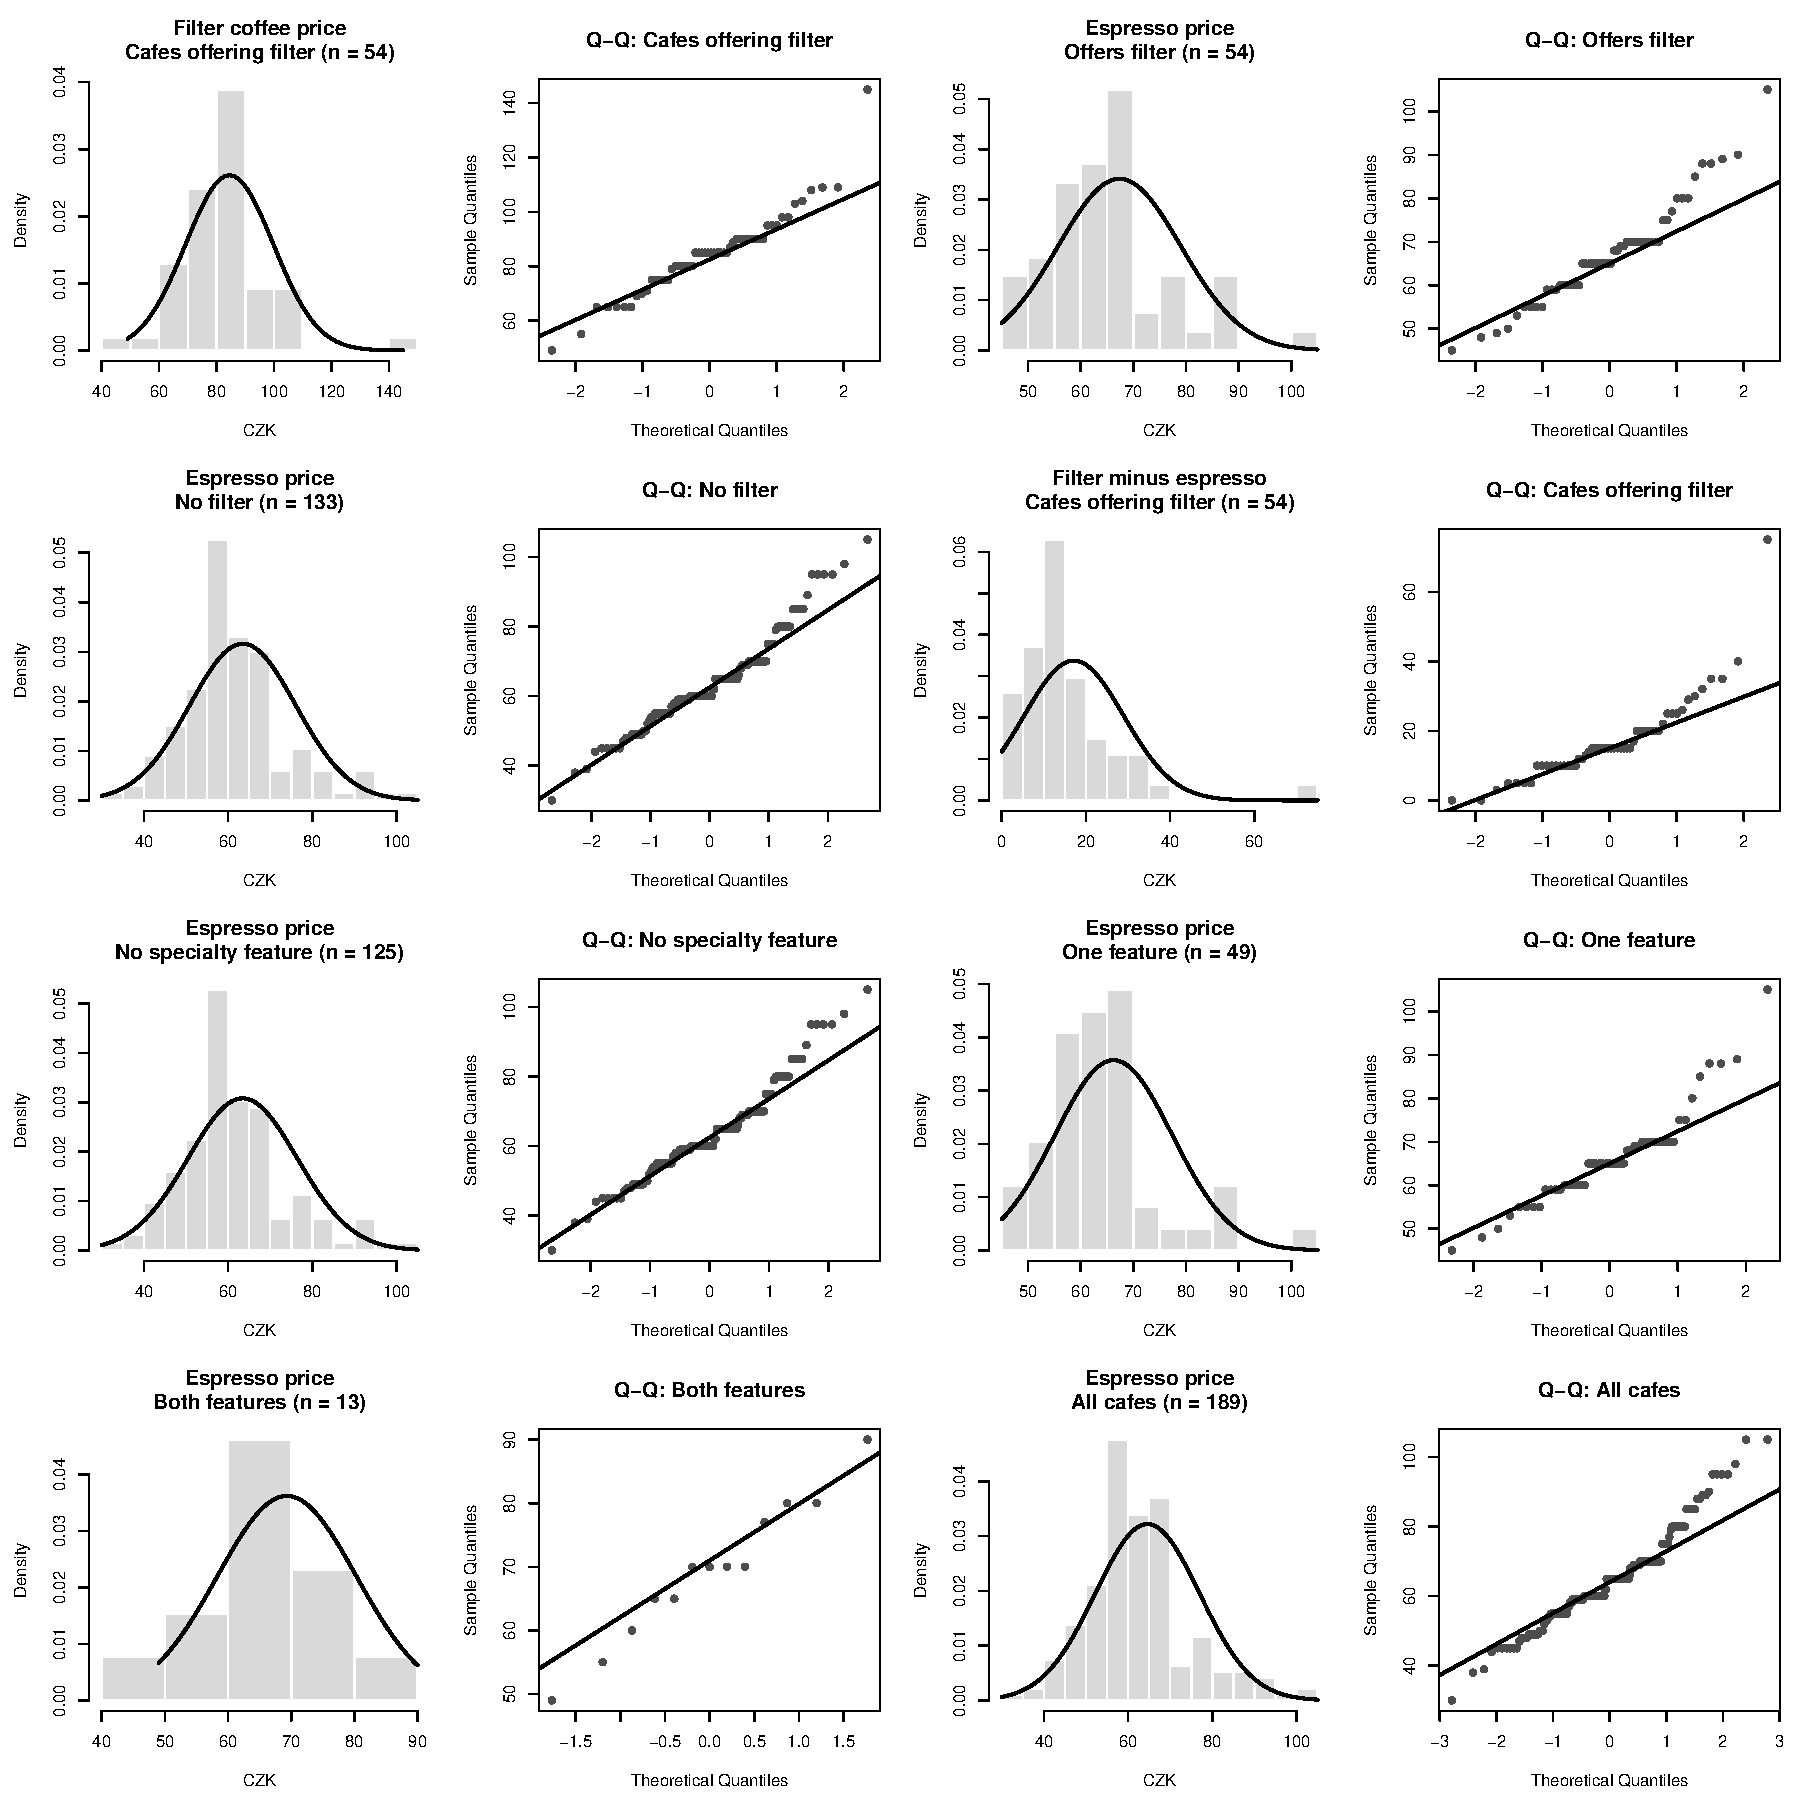
\includegraphics[width=\textwidth]{distributions.pdf}
\caption{Histogram with the normal curve of the same mean and SD, and normal Q--Q plot, for each row of Table~\ref{tab:decision} (prices in CZK; group sizes in the panel titles).}
\label{fig:distributions}
\end{figure}

\begin{figure}[H]
\centering
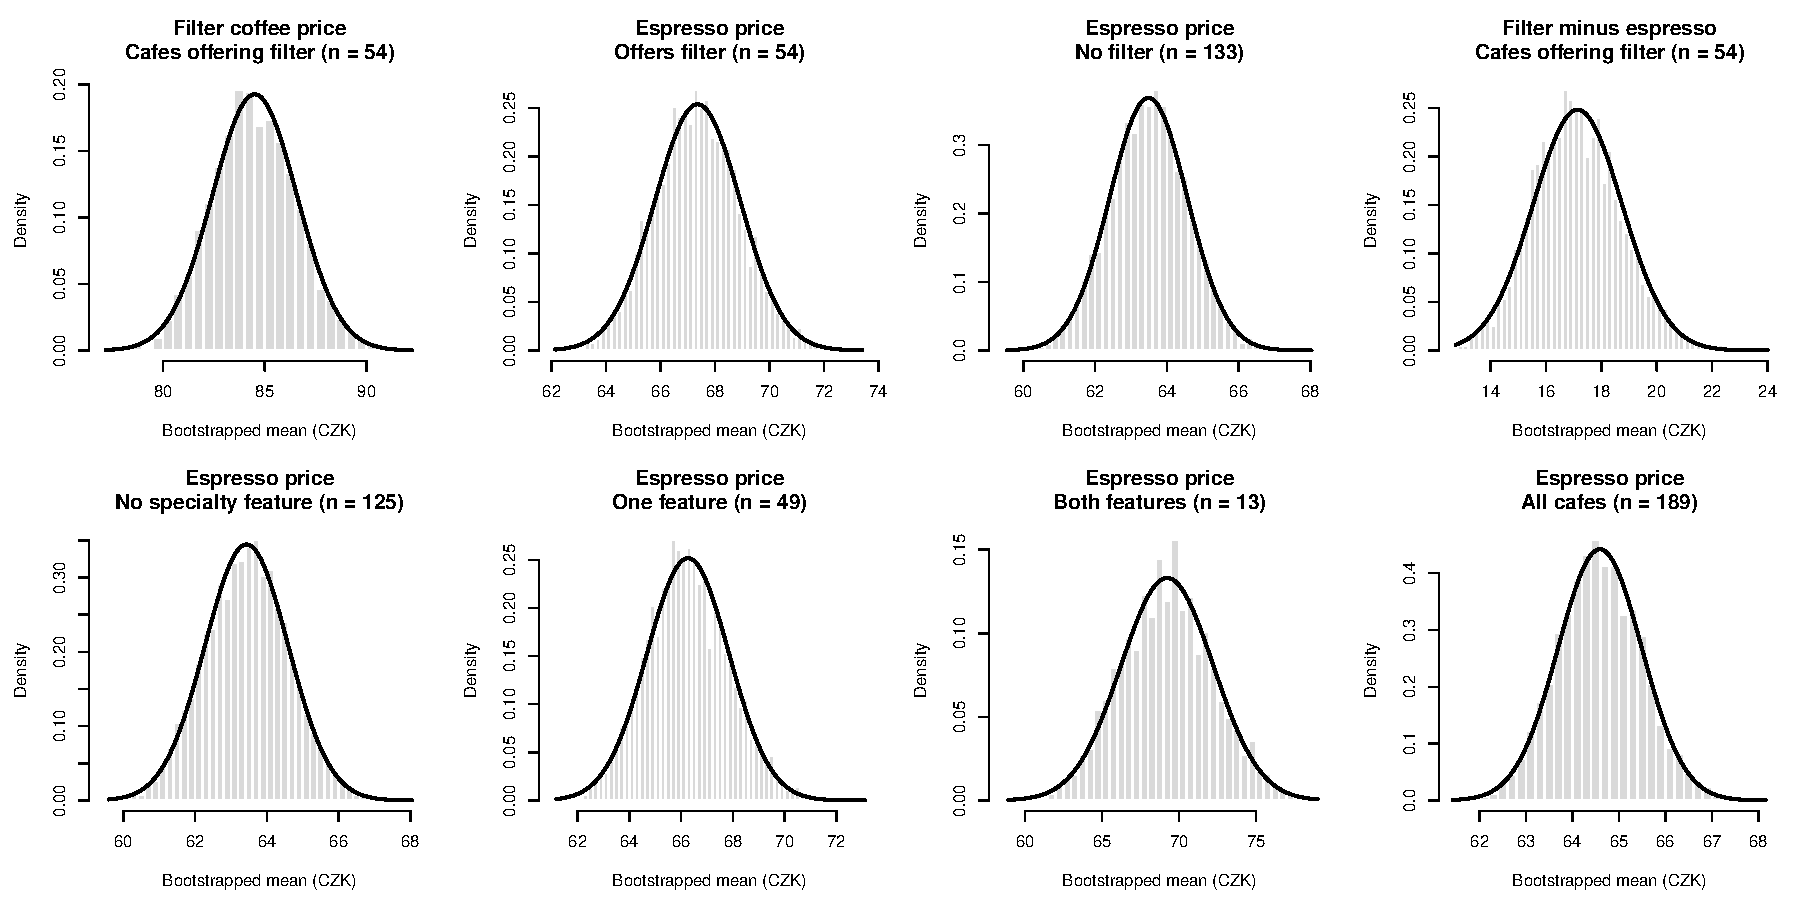
\includegraphics[width=\textwidth]{D_bootstrap_means.pdf}
\caption{Distribution of \Boot{} bootstrapped means for each row of Table~\ref{tab:decision} (CZK), with the normal curve. Near-normal shapes show that the central limit theorem applies.}
\label{fig:bootmeans}
\end{figure}

\begin{figure}[H]
\centering
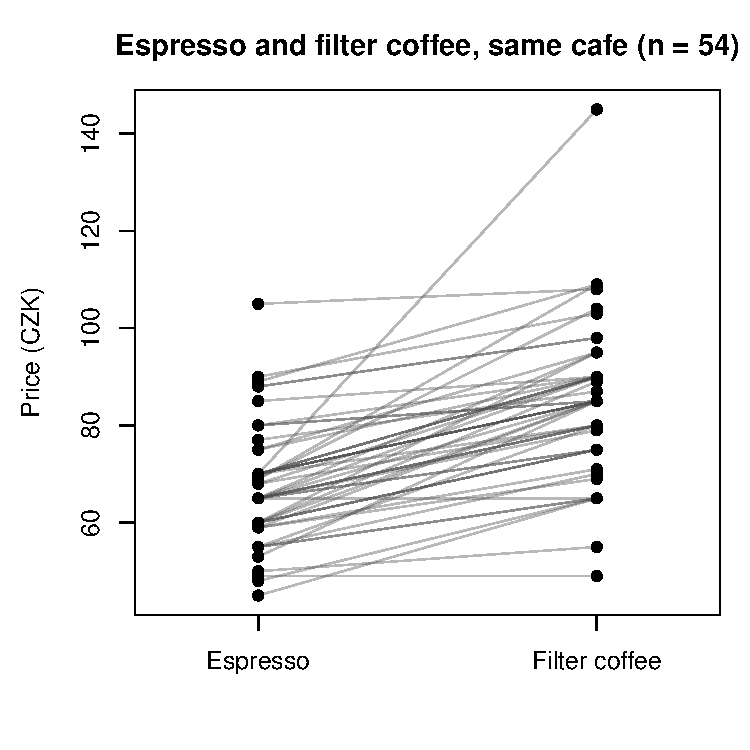
\includegraphics[width=0.5\textwidth]{D_paired_prices.pdf}
\caption{Espresso and filter coffee price (CZK) in each of the \Nfilter{} caf\'es that sell both; lines connect the two prices of one caf\'e.}
\label{fig:paired}
\end{figure}

\section{Regression diagnostics}\label{app:diagnostics}

Figure~\ref{fig:diag} shows the residuals of the three linear models and Table~\ref{tab:influence} the influential observations. In none of the models do the residuals curve against the fitted values, and the Breusch--Pagan tests do not indicate unequal spread (A7 $p = \BPseven$, A8 $p = \BPeight$, A9 $p = \BPnine$); HC3 standard errors are used anyway. The residuals of A7 and A9 have a slightly long right tail from a few expensive filter coffees, and those of A8 inherit the right skew of espresso prices; with $n \ge 54$ this does not threaten the intervals. The variance inflation factors are at most \AnineVIF. Caf\'es with Cook's distance above $4/n$ were removed one model at a time: every key estimate keeps its sign and size and stays significant (Table~\ref{tab:influence}), so no conclusion depends on a few caf\'es.

\begin{figure}[H]
\centering
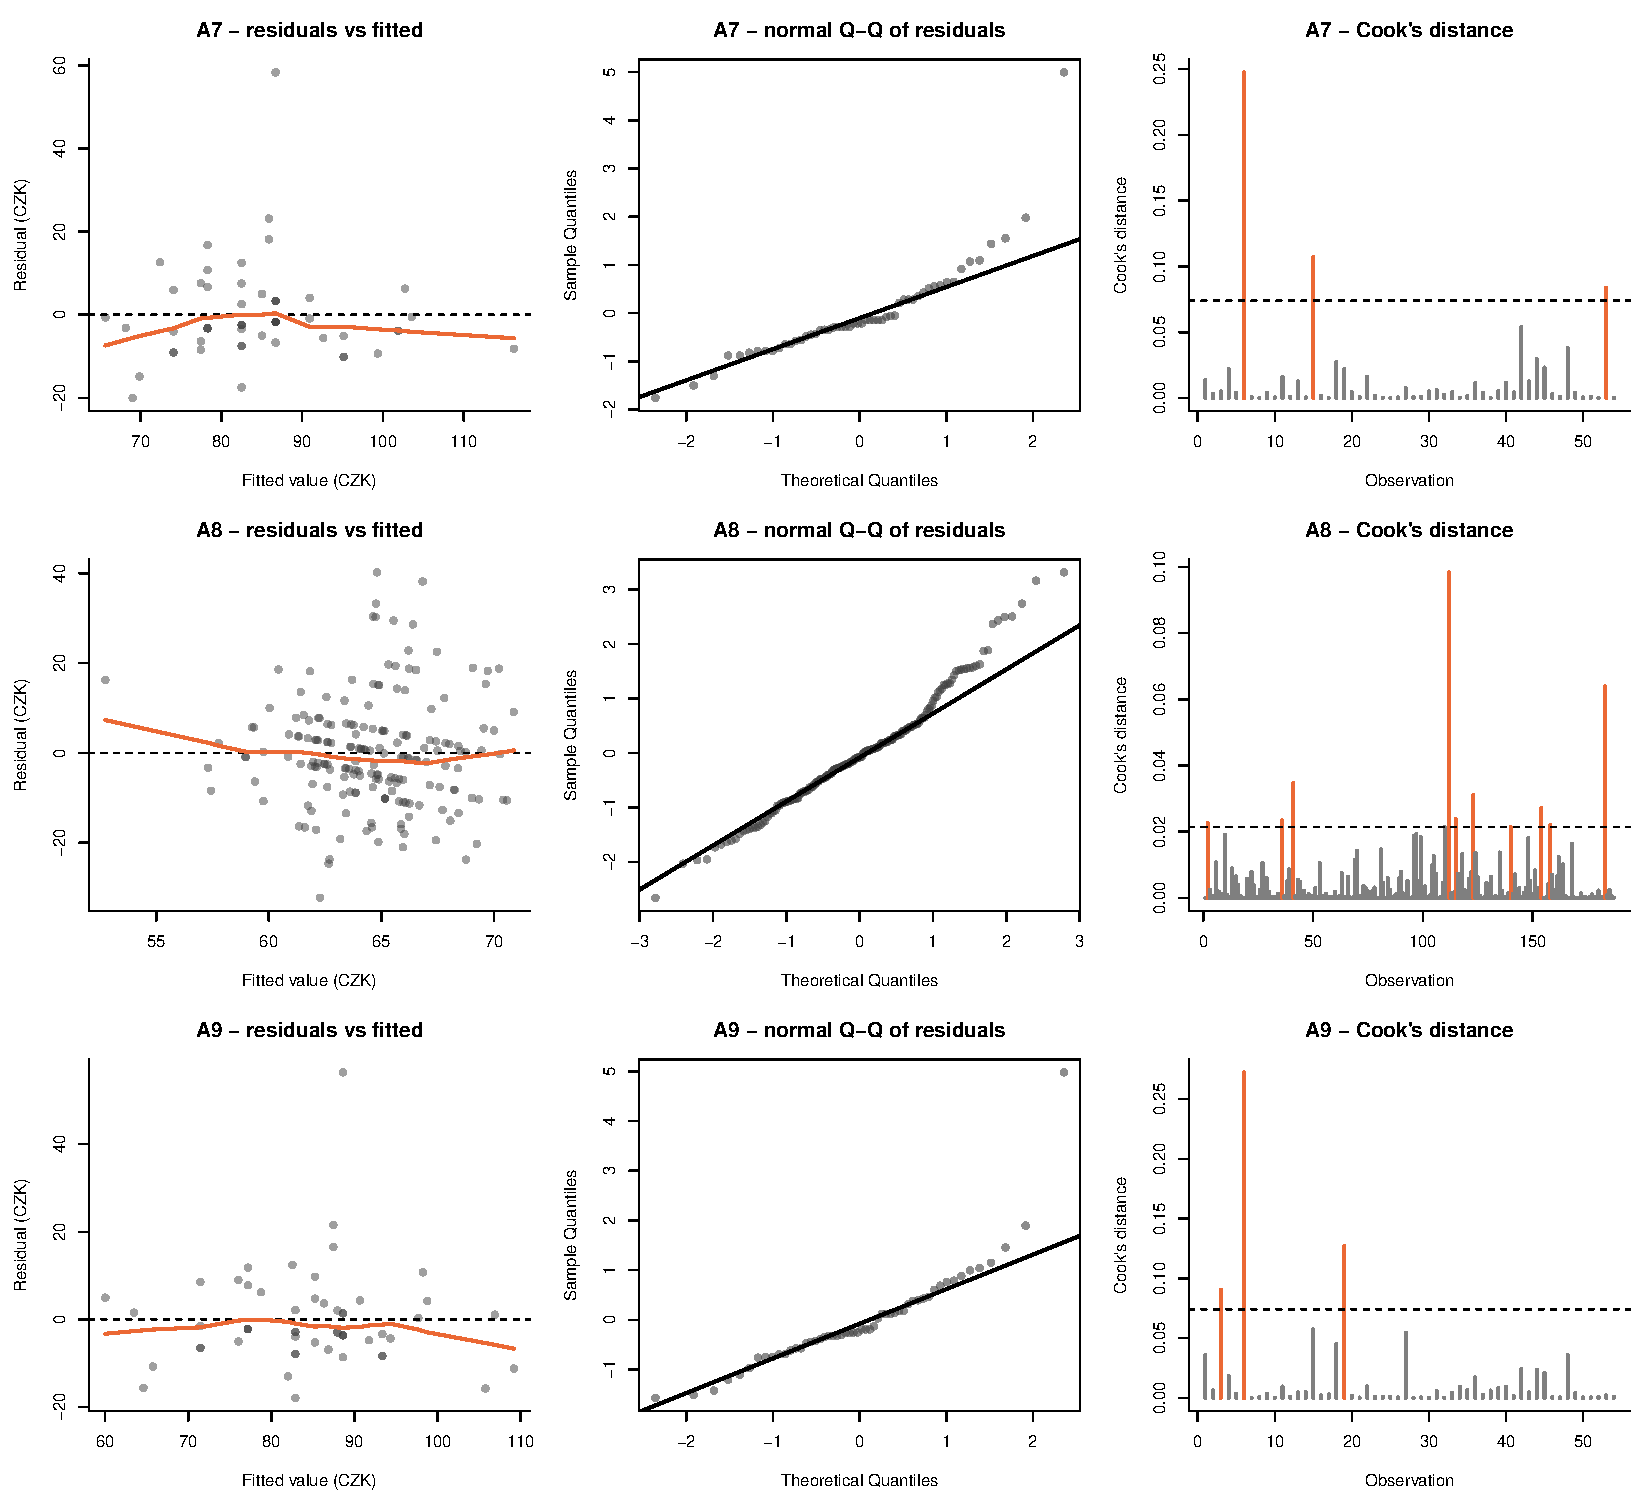
\includegraphics[width=\textwidth]{C_diagnostics.pdf}
\caption{Diagnostics of the linear models A7, A8 (Model~2) and A9: residuals against fitted values with a lowess smoother (left), normal Q--Q plot of the standardised residuals (middle), and Cook's distance with the cut-off $4/n$ (right; orange bars exceed it).}
\label{fig:diag}
\end{figure}

\begin{table}[H]
\centering\small
\caption{Influential observations, variance inflation factors, and the key estimate of each model with all caf\'es and without those with Cook's $D > 4/n$ (A7: slope per 10\,CZK; A8: filter gap in CZK; A9: interaction; A10: average marginal effect in percentage points).}
\label{tab:influence}
\fittable{C_influence.tex}
\end{table}

\section{Alternative tests and robustness}\label{app:robustness}

The checks in this appendix were \emph{not planned in advance}; they are exploratory and do not replace the primary results in Section~3. Table~\ref{tab:robustness} lists a second method for every question. The rank-based tests, bootstrap intervals and alternative specifications agree with the primary method for eight questions. For A4, Welch's and the classic ANOVA find no difference but Kruskal--Wallis does ($p = .040$); the rank test compares the whole distributions, and the right tail of the ``one feature'' group pulls the means less apart than the ranks. For A9, the robust test gives $p = .048$ and the classic test $p = .051$: the result is on the threshold. For A3, removing the most extreme caf\'e gives a mean difference of \AthreeTrim\,CZK. For A8, a log of distance gives a filter gap of \AeightLog. Table~\ref{tab:posthoc} gives the full A4 post hoc comparisons. Table~\ref{tab:holm} adjusts the ten primary $p$-values with Holm's method: \HolmSig{} of the \RawSig{} significant results remain (A3, A5, A6, A7).

\begin{table}[H]
\centering\small
\caption{Second method for every question and whether it agrees with the primary method at $\alpha = .05$. Intervals are 95\%; bootstrap intervals use \Boot{} resamples (seed \Seed).}
\label{tab:robustness}
\fittable{D_robustness.tex}
\end{table}

\begin{table}[H]
\centering\small
\caption{A4: all pairwise comparisons of the mean espresso price (CZK) between caf\'es with none, one or both specialty features. Differences with 95\% simultaneous confidence intervals and adjusted $p$-values; the Wilcoxon rank-sum $p$-values are Holm-adjusted.}
\label{tab:posthoc}
\fittable{D_posthoc.tex}
\end{table}

\begin{table}[H]
\centering\small
\caption{Primary $p$-values of the ten analyses and Holm-adjusted $p$-values (family of ten tests).}
\label{tab:holm}
\begin{tabular}{lrrc}
\toprule
Analysis & Primary $p$ & Holm-adjusted $p$ & Significant after adjustment? \\
\midrule
A1 & .321 & .321 & No \\
A2 & .023 & .115 & No \\
A3 & < .001 & < .001 & Yes \\
A4 & .136 & .273 & No \\
A5 & < .001 & .003 & Yes \\
A6 & < .001 & < .001 & Yes \\
A7 & < .001 & < .001 & Yes \\
A8 & .024 & .115 & No \\
A9 & .048 & .145 & No \\
A10 & .015 & .091 & No \\
\bottomrule
\end{tabular}

\end{table}

\section{Reproducibility}\label{app:reproducibility}

{\raggedright Repository: \url{https://github.com/aidanosbaugh/data-analytics-semestral-project}. Run, from the repository root, \texttt{analysis/01\_cleaning.R} (raw data $\to$ \texttt{dataset.csv} and the cleaning table), \texttt{analysis/02\_descriptive.R} (descriptive statistics, distribution checks, decision table) and \texttt{analysis/03\_analysis.R} (hypotheses, A1--A10, robustness, diagnostics, and \texttt{tables/results\_macros.tex} with every number quoted in the text); then compile \texttt{report/report.tex}. Software: R~\Rversion; the cleaning and descriptive scripts use base R only, the analysis uses \texttt{sandwich}~\Versandwich, \texttt{lmtest}~\Verlmtest, \texttt{car}~\Vercar{} and \texttt{marginaleffects}~\Vermarginaleffects. Every bootstrap uses seed \Seed{} and \Boot{} resamples.\par}

\end{document}
